\documentclass[10pt,twocolumn,letterpaper]{article}
\usepackage[review]{cvpr}
\usepackage{times,graphicx,amsmath,amssymb,booktabs,microtype}
\usepackage[accsupp]{axessibility}
\definecolor{cvprblue}{rgb}{0.0,0.447,0.698}
\usepackage[pagebackref,breaklinks,colorlinks,allcolors=cvprblue]{hyperref}
\def\paperID{*****}
\def\confName{CVPR}
\def\confYear{2027}
\newcommand{\paths}{\mathcal C}
\newcommand{\edges}{\mathcal E}
\title{Task Information Audits for Connectome Graph Interventions}
\author{Anonymous CVPR submission}
\begin{document}
\maketitle
\begin{abstract}
Removing a circuit motif need not remove the computation it supports. On the
Drosophila MaleCNS connectome, two reconstructed graph interventions preserve
identical degree and module-pair statistics while eliminating all designated
common-relay triples. Yet one retains both task sources and the other loses
access to one, consistent with archived classification accuracies of 97.45\%
and 50.55\%. Readout retraining on the reconstructed transfers reproduces this
high-versus-chance contrast, without recovering the identical historical run
instances. To explain what survives a graph intervention, we introduce
task-information auditing, which separates structural constraints, information
available at the readout, and finite-model behavior through a compact
source-to-readout transfer matrix. For a fixed two-step nonnegative linear
propagator, we prove that perfect Bayes solvability of a noiseless subspace
XOR task requires neither a common relay nor full transfer rank, but exactly
the visibility of both sources. Across two additional graph extractions, ideal
solvability remains perfect at every nonzero intervention dose, even as
trained accuracy rises from approximately 67\% to 94\%. In a four-source
CIFAR-10 probe, an independent transfer direction accompanies an increase in
target-source classification accuracy from 16.4\% to 56.6\%. These findings
shift the evaluation of graph interventions from the structures they preserve
to the task-relevant computations they leave intact.
\end{abstract}

\begin{figure*}[t]
\centering
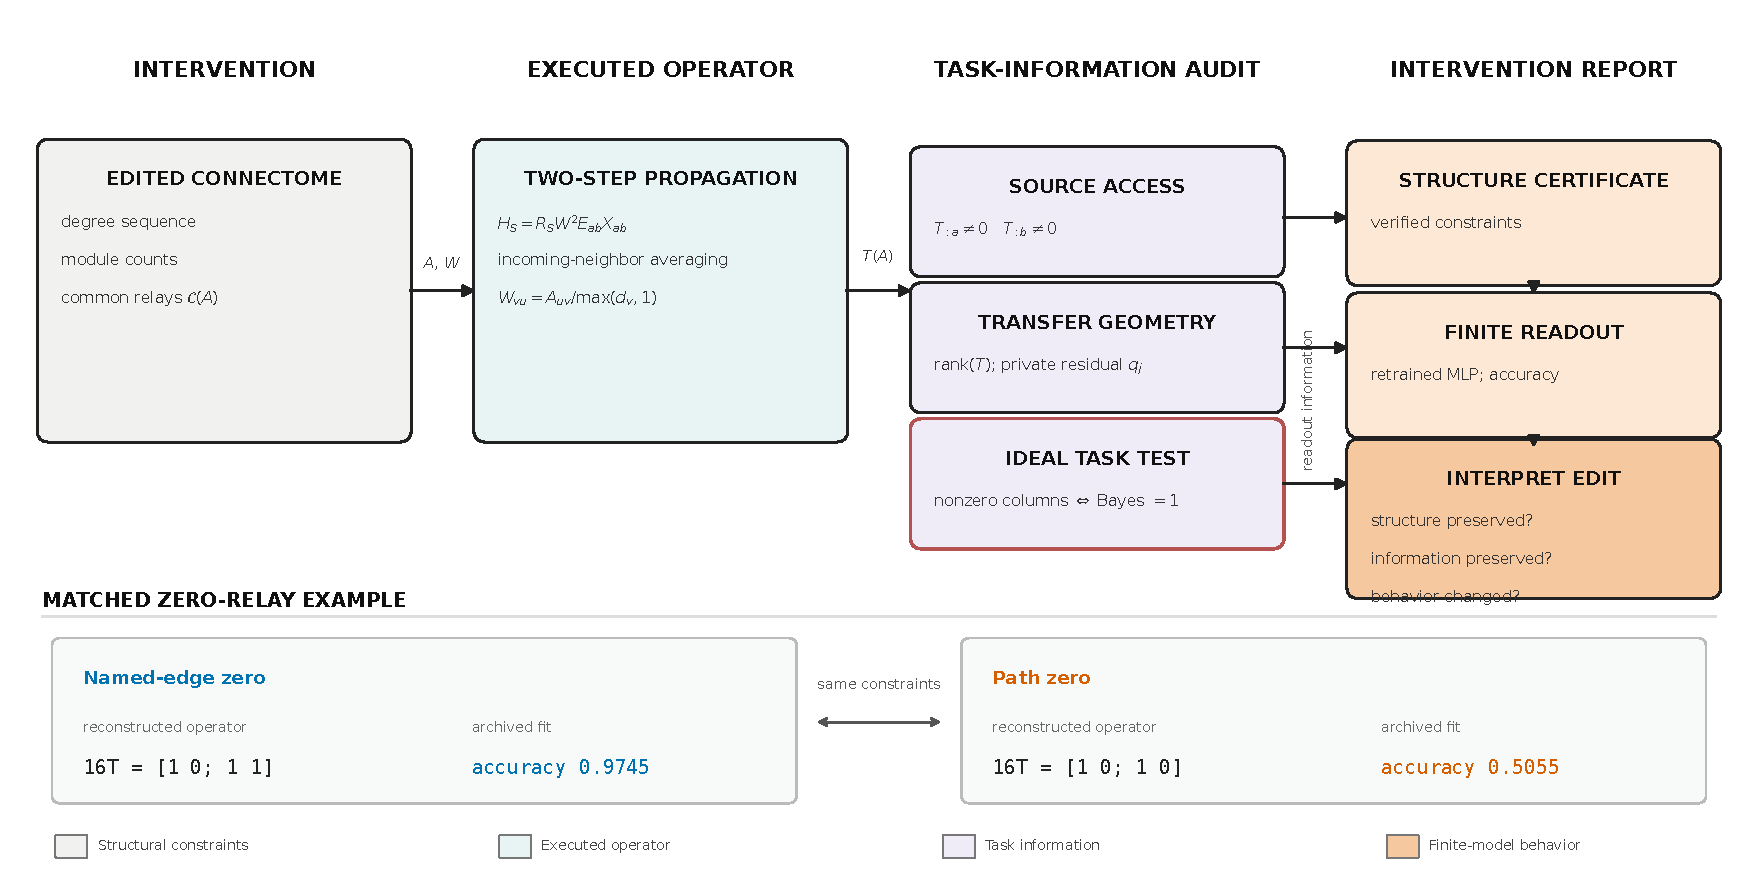
\includegraphics[width=0.78\textwidth]{figures/overview.pdf}
\caption{\textbf{Identical structural constraints do not imply identical task
information.} Both reconstructed interventions preserve the original degree
sequences and module-pair counts and eliminate all common-relay triples.
Named-edge compensation retains both sources through separate relays, whereas
path conditioning leaves source $b$ with no two-hop route to the selected
readout. Only contributing two-hop routes are shown. Transfer matrices are
reconstructed; accuracies are corresponding archived outcomes.}
\label{fig:overview}
\end{figure*}

\section{Introduction}
\label{sec:introduction}

When a graph intervention removes a circuit motif, what exactly has been
removed from the computation? Figure~\ref{fig:overview} illustrates why the
answer cannot be inferred from the edited structure alone. Two reconstructed
interventions on a fly connectome satisfy identical degree and module-pair
constraints and eliminate all common-relay triples for the designated sources
and sinks. Nevertheless, one retains both sources through separate relays,
while the other loses access to one. Their corresponding archived classifiers
achieve 97.45\% and 50.55\% accuracy. The structural certificates agree, but
the task information reaching the readout does not.

Degree-preserving rewiring and motif deletion isolate structural properties,
but a compensating edit can introduce replacement routes. The absence of a
motif therefore does not establish the absence of the associated computation.
The relevant object is the signal that the executed operator delivers to the
readout.

We address this gap with a task-information audit that separates three
questions: whether the declared structural constraints hold, whether the
information required by the task reaches the readout, and how effectively a
finite model uses that information. For the fixed two-step linear operator
studied here, propagating basis signals from the designated sources produces
a compact source-to-readout transfer. Its columns capture source access, and
their geometry describes how sources are mixed. Unlike a motif count, the
transfer includes every contributing route under the operator used by the
classifier.

The audit yields an exact result for the noiseless subspace XOR task: perfect
Bayes accuracy is possible if and only if both source columns are nonzero.
Neither a shared relay nor full transfer rank is required. Separate routes
can therefore preserve the task after a targeted common relay disappears.
Applied to the reconstructed MaleCNS interventions, the criterion
distinguishes the information-preserving and information-losing zero-relay
graphs, consistent with their archived outcomes.

A second distinction remains even when ideal task information survives.
Across two $k{=}8$ extractions, every nonzero dose retains both sources and
therefore preserves perfect Bayes solvability, yet finite-readout accuracy
rises from roughly 67\% to 94\%. Structural preservation, information
availability, and learned performance are different levels of evidence. On
visual parity and four-image CIFAR-10 probes, source mixtures and private
transfer directions further show why a visible source need not be equally
usable by a trained readout.

Our contributions are threefold:
\begin{itemize}
  \item We formulate a task-information audit that separates structural
        constraints, source-to-readout information, and finite-model
        behavior, with an exact criterion for a specified noiseless task.
  \item We identify a matched-connectome counterexample in which
        eliminating common relays can either preserve or remove the source
        information required by the task.
  \item We distinguish ideal information preservation from finite-readout
        performance and extend the audit to source recovery and mixing
        geometry in visual probes.
\end{itemize}

\section{Related Work}
\label{sec:related}

\paragraph{Connectome-constrained computation.}
Large-scale fly connectomes support models constrained by measured neuronal
wiring~\cite{dorkenwald2024,malecns2026}. Lappalainen et
al.~\cite{lappalainen2024} combine connectomic constraints with task training
to predict neural responses across the visual system. Structure-only models
investigate visual computation under fixed wiring and wiring-cost
comparisons~\cite{structure2026}. Beiran and Litwin-Kumar~\cite{beiran2025} characterize dynamical
degeneracy under fixed connectomic weights and show how partial activity
recordings can resolve it. Our question concerns the source information
left by an intervention in a fixed computational model.

\paragraph{Null models and structural attribution.}
Degree-preserving swaps and motif counts are established tools for network
analysis~\cite{maslov2002,milo2002}; weighted-network randomization further
shows that degree and strength are different constraints~\cite{milisav2025}.
Dhiman~\cite{dhiman2026} studies staged controls for initialization, degree,
and early optimization in connectome-constrained networks. Park~\cite{park2026}
shows that standard randomizations introduce sensory--motor shortcuts in
embodied agents and evaluates boundary-preserving controls, graded shortcut
doses, and sham interventions. These controls diagnose task-relevant routes
at the level of the chosen graph edit. Our audit adds the executed operator:
it separates the declared structural constraint from the source information
that reaches the readout, including separate-relay routes that survive a
zero common-relay count.
Zhang et al.~\cite{zhang2025motifs} analyze how coherent and incoherent
motifs affect representational capacity and stability; our question is
whether removing a declared motif removes the inputs required by a task.

\paragraph{Graph communication and rewiring.}
Curvature-based analysis~\cite{curvature2022} and joint width--depth--topology
analysis~\cite{oversquashing2023} relate graph structure to information
transport. Spectral pruning demonstrates that removing edges can improve
communication and generalization~\cite{pruning2024}, while virtual-node
rewiring creates efficient long-range routes~\cite{virtual2024}.
GraphGPS combines local and global communication~\cite{graphgps2022};
oversmoothing itself depends on the model's parameter
regime~\cite{phase2024}. We fix the two-step propagator and evaluate what task information its
structural interventions preserve, complementing methods that alter
communication to improve learning.

\paragraph{Evaluating explanations through interventions.}
GNNExplainer uses subgraphs and features to explain learned
predictions~\cite{gnnexplainer2019}. ROAR shows that deletion-based image
attribution is confounded by distribution shift and evaluates removal with
retraining~\cite{roar2019}. RegExplainer identifies task and distribution
mismatch in graph-regression explanations~\cite{regexplainer2024}.
These works establish that an evaluator must match the intervention and the
task. Graph compensation creates a related but distinct problem: preserving
degree while removing an edge can introduce a replacement computation.
Our transfer audit evaluates the computation that replaces the removed one.

\section{Task-Information Audit}
\label{sec:method}

A graph intervention changes wiring; its interpretation depends on the
computation that remains. We audit an intervention at three levels. First, we
verify the structural properties the edit claims to preserve. Second, we
examine which task-relevant source signals reach the readout under the
executed operator. Third, we evaluate how a finite trained model uses the
resulting representation. These levels answer different questions and are not
interchangeable evidence.

\subsection{Specify the executed computation}
\label{sec:operator}

For a fixed linear propagation prefix, source-to-readout transfer can be
computed directly, without training a classifier or enumerating every source
input. The audit takes four inputs: an edited graph, its executed propagation
operator, designated task sources, and readout locations.
Let $A_{uv}=1$ denote a directed edge $u\!\to\!v$. The main experiments
use binary support and incoming-neighbor averaging,
\begin{equation}
 d_v=\sum_u A_{uv},\qquad
 W_{vu}=\frac{A_{uv}}{\max(d_v,1)}.
 \label{eq:operator}
\end{equation}
Rows for zero in-degree remain zero. Features propagate linearly for two
rounds, $H=W^2X$, before an MLP reads the concatenated features at
$S=\{s_1,s_2\}$. The operator direction, normalization, and readout
locations are part of the computational model.

With nonzero features only at sources $a,b$, let $E_{ab}$ place the source
vectors and $R_S$ select the sinks. The graph affects the classifier input
through
\begin{equation}
 H_S=T(A)X_{ab},\qquad T(A)=R_SW(A)^2E_{ab}.
 \label{eq:transfer}
\end{equation}
$T$ has two source columns and two sink rows. It records every two-step
route contributing to these inputs, including routes outside a selected
motif family. Equal $T$ matrices give identical readout inputs for any
source features; equal graph statistics need not. Computing $T$ requires
propagating two basis columns, rather than constructing all entries of
$W^2$. For a sparse fixed operator and $h$ steps, this costs
$O(h|E|\,n_{\rm source})$ time and $O(Nn_{\rm source})$ storage.

For this operator, every entry has an explicit path interpretation:
\begin{equation}
 T_{sj}=\sum_r W_{sr}W_{rj}
 =\sum_r\frac{A_{jr}A_{rs}}{\max(d_r,1)\max(d_s,1)}.
 \label{eq:pathsum}
\end{equation}
Each term is one source--relay--sink route. A common-relay count records
only routes shared by both sources. Equation~\eqref{eq:pathsum} also retains
separate-relay routes and their weights. This is why equal degree, module
and common-relay statistics need not imply equal readout inputs.

\subsection{Read the transfer at three levels}
\label{sec:observability}

\paragraph{Source access is not source recovery.}
Source visibility is weaker than source recovery, and neither alone determines an arbitrary trained classifier. For the noiseless XOR task considered here, visibility is nevertheless an exact criterion for whether the label remains recoverable. A source is \emph{visible} when its column of $T$ is nonzero. Visibility
means that some source-dependent signal reaches the readout; it does not
mean that the source vector can be reconstructed. Full column rank is
the stronger linear-separability condition for independent sources.

\paragraph{Ideal task information.}
For the archived subspace task, visibility is already an exact criterion.
Let $c_a,c_b$ be independent balanced bits and
$x_a=P_{c_a}z_a$, $x_b=P_{c_b}z_b$, with independent
$z_a,z_b\sim\mathcal N(0,I_8)$. The class subspaces
$U_c=\operatorname{span}(P_c)\subset\mathbb R^{16}$ satisfy
$U_0\cap U_1=\{0\}$, and the label is $y=c_a\oplus c_b$.

\noindent\textbf{Proposition 1 (ideal population criterion).}
\emph{For a fixed nonnegative $T$ and no other active inputs, the Bayes
accuracy from $H_S=TX_{ab}$ is}
\begin{equation}
 \operatorname{Acc}^{*}(T)=
 \begin{cases}
  1, & T_{:a}\ne0\ \text{and}\ T_{:b}\ne0,\\
  \tfrac12, & \text{otherwise}.
 \end{cases}
 \label{eq:criterion}
\end{equation}

\emph{Proof.} If $T_{:b}=0$, the readout is independent of $c_b$,
so $\Pr(y=1\mid H_S)=1/2$; the same holds for $a$.
If both columns are nonzero, summing sink vectors gives
$z=\alpha x_a+\beta x_b$, where
$\alpha=\sum_sT_{sa}>0$ and $\beta=\sum_sT_{sb}>0$.
For equal source classes, $z\in U_0\cup U_1$. For different classes,
transversality and nonzero Gaussian coordinates imply
$z\notin U_0\cup U_1$ almost surely. Subspace membership therefore
recovers the XOR label. $\square$

Rank-one transfer can thus retain ideal task information: two nonzero
parallel columns still supply both class-dependent terms. A common relay
is likewise unnecessary because separate routes can expose both sources.
The supplement gives the full argument and ten-seed basis-rank check.
The proposition is a population statement for this noiseless task, not a
prediction of finite-sample optimization or a guarantee of source recovery.

\paragraph{Multi-source mixing geometry.}
With $m$ designated active sources, the same linear prefix gives
$H_S=TX$: each column of $T$ belongs to one source and each row of $X$
holds that source's features. For a target source $j$, let $t_j=T_{:j}$
and let $T_{-j}$ collect the other columns. Its private component is the
residual after projecting out those columns:
\begin{equation}
 q_j=(I-P_{\operatorname{span}(T_{-j})})t_j,\qquad
 \rho_j=\|q_j\|_2^2.
 \label{eq:private}
\end{equation}
Because $q_j$ is orthogonal to every other column,
$q_j^\top H_S=\rho_j x_j$ under noiseless mixing. If $\rho_j>0$,
$x_j=q_j^\top H_S/\rho_j$ recovers the target without reconstructing the
other sources. A zero residual means no linear projection isolates it from
arbitrary competing features. That is source recovery, not label solvability:
class information can remain when exact separation is impossible.

\subsection{What the structural interventions constrain}
\label{sec:paths}

The graph controls preserve each node's in-/out-degree and module-pair
edge counts. For fixed sources and sinks, a common-relay family is
\begin{equation}
 \mathcal C(A)=\{(r,s):s\in S,\ A_{ar}A_{br}A_{rs}=1\}.
 \label{eq:paths}
\end{equation}
A member represents two source edges converging at a relay and one edge
to a sink. Its three-edge description omits separate-relay routes.
The number of named motif edges retained is an even narrower statistic.
Neither quantity specifies all columns of Eq.~\eqref{eq:transfer}.

We compare two archived intervention designs. Named-edge compensation
removes selected motif edges and replaces each through a module-matched
double-edge swap
$(u\!\to\!v,x\!\to\!y)\mapsto(u\!\to\!y,x\!\to\!v)$.
Matching source-module and target-module labels preserves module counts;
the exchange preserves every labeled degree. It does not constrain
other source-specific routes.

The path-conditioned design retains a prefix of $\mathcal C$, protects its
path-edge union and rejects swaps that create new members. Other edges
are processed in sorted order with randomized feasible partners. This is
a common-relay constraint, not a complete source-transport constraint.

Degree nulls rewire the whole dose graph. Protected nulls retain selected
path edges while rewiring the background without the no-new-relay rule.
The two therefore ask different counterfactual questions.

\subsection{Turn the analysis into an audit}
\label{sec:controls}

The procedure has four steps. First, verify the declared structural
invariants. Second, construct $T$ from the actual direction, normalization,
propagation depth and sinks. Third, report visibility, the applicable
ideal-task criterion, and, for competing sources, rank and private
components. Finally, compare finite readouts against these information-level
predictions. An oracle given both sources tests label learnability;
$W=I$ prevents cross-node transport; linear-readout, shuffled-label and
moved-readout controls test alternative explanations.

The output pairs a structural certificate with a statement about task
information and a separate measurement of finite-model behavior.

The audit does not replace structural controls. It tests whether those
controls support the task-level conclusion drawn from them. The exact matrix
reduction applies to a fixed linear propagation prefix. Nonlinear message
passing, gating and spiking dynamics require an input-dependent analysis of
source access.

\section{Experiments}
\label{sec:experiments}

\subsection{Tasks, graphs, and statistical units}
\label{sec:setup}

\paragraph{A task with known source information.}
Each source independently receives a balanced binary class $c_a,c_b$.
For class $c$, its 16-dimensional feature is $P_cz$, where
$z\sim\mathcal N(0,I_8)$ and $P_c$ is an orthonormal basis for a fixed
eight-dimensional subspace. The two class bases are drawn separately for
each seed block and are not required to be mutually orthogonal. All
non-source features are zero. The label is $y=c_a\oplus c_b$.
After two rounds of Eq.~\eqref{eq:operator}, a
$32\!\to\!64\!\to\!1$ ReLU MLP reads the two concatenated sink features.
No nonlinear message-passing layer precedes this readout.

The archived protocol fixes ten seed blocks
$\{11,17,23,31,41,53,67,79,97,103\}$. Each defines the subspace bases,
an on-the-fly training stream, and a separate 2,048-example evaluation
stream. Readouts are trained for 120 epochs of 32 batches of 128 samples
using Adam with learning rate 0.006. The ordinary graph conditions share
the data streams within each seed block. They are retrained separately,
so the evaluation measures finite-readout performance after an intervention.
The readout is constructed before an in-function seed reset; pairing the
data streams does not establish identical initial parameter values.

\paragraph{Controlled and biological wiring.}
The controlled graph contains 96 nodes and 337 directed edges. Its two
sources connect only to a designated relay; the relay is the only
incoming route to the two sinks. Background edges are generated outside
these restricted destinations. Removing the four motif edges therefore
eliminates source-to-sink communication under two-step propagation.

The real graphs are extracted from the public MaleCNS v1.0
connectome~\cite{malecns2026}. Visual annotation predicates define a
candidate neuron set; the 768 highest-total-degree neurons are selected,
then each target retains its highest-weight incoming partners. The
propagator uses the resulting binary support. Table~\ref{tab:graphs}
keeps the extraction settings separate. A relay is selected
deterministically from ascending node indices with two source neighbors,
two sink neighbors, five distinct nodes, and no direct source--sink edges
in the dense extracted graph. For the two $k=8$ extractions, the first
candidate with at least three common-relay triples is selected. This
criterion ensures distinct doses rather than selecting by accuracy.

\begin{table}[t]
\centering
\caption{\textbf{Real-wiring cohorts.} Each contains 768 nodes.
$k$ is the maximum number of retained incoming edges.
The broad and narrow $k=8$ node sets overlap in 195 neurons; all derive
from one male connectome.}
\label{tab:graphs}
\small
\begin{tabular}{lrrr}
\toprule
Extraction & Candidate IDs & $k$ & Edges \\
\midrule
Narrow, initial & 29,534 & 4 & 3,072 \\
Broad & 105,275 & 8 & 6,141 \\
Narrow & 29,534 & 8 & 6,144 \\
\bottomrule
\end{tabular}
\end{table}

\paragraph{Reporting convention.}
Intervals are 5,000-resample bootstrap 95\% intervals over the ten seed
blocks. Real-graph comparisons use paired sign-flip tests with
Benjamini--Hochberg correction~\cite{benjamini1995}. Reconstructed matrices
and archived accuracies are distinct evidence layers; hashes and seeds are
recorded in the supplement.

\subsection{Calibrating a known structural effect}
\label{sec:calibration}

Before examining biological wiring, we use a graph in which the targeted
circuit is the only source-to-readout route. This checks that the task,
operator, and readout respond when that access is removed. Table~\ref{tab:calibration} shows the
controlled-graph result. The graph reaches 99.71\% accuracy and the oracle
99.91\%. A degree-preserving null reduces accuracy to 50.17\%, whereas
protecting the four route edges retains 99.71\%. Deleting the motif,
removing cross-node propagation, or moving the readout produces chance
performance. The paired intact-minus-no-cross-node difference is
$0.4954$ with interval $[0.4862,0.5021]$.

\begin{table}[t]
\centering
\caption{\textbf{Controlled calibration.} Ten seed blocks on the
96-node, 337-edge graph. Intervals are bootstrap 95\% intervals for mean
accuracy. The protected null fixes the four route edges while rewiring
the background.}
\label{tab:calibration}
\small
\begin{tabular}{lcc}
\toprule
Condition & Accuracy & 95\% interval \\
\midrule
Intact graph & 0.9971 & [0.9963, 0.9979] \\
Protected null & 0.9971 & [0.9962, 0.9979] \\
Degree null & 0.5017 & [0.4945, 0.5111] \\
No cross-node propagation & 0.5017 & [0.4945, 0.5113] \\
Motif edges removed & 0.5017 & [0.4946, 0.5108] \\
Readout moved & 0.5017 & [0.4943, 0.5113] \\
Linear readout & 0.4983 & [0.4904, 0.5075] \\
Shuffled training labels & 0.4918 & [0.4841, 0.4990] \\
Oracle source readout & 0.9991 & [0.9983, 0.9997] \\
\bottomrule
\end{tabular}
\end{table}

The controlled deletion removes the only source-to-sink route. Deleting
the same kind of motif in a larger connectome need not remove the
task-relevant computation.

\subsection{Named edges do not define the intervention}
\label{sec:edge}

On the initial narrow $k=4$ subgraph, the selected motif consists of
$a\!\to\!r$, $b\!\to\!r$, $r\!\to\!s_1$, and
$r\!\to\!s_2$. The edge-conditioned design requests retention in that
order and replaces deleted edges with module-matched swaps. It preserves
degree and module counts, without checking the common-relay family after
each exchange.

The controlled result does not extend automatically to a compensated edit.
Figure~\ref{fig:edge-path}a exposes the resulting mismatch. Intact accuracy
is $0.9772$, while the zero-named-edge graph achieves $0.9745$.
The paired difference is $0.0027$ with interval $[-0.0031,0.0078]$.
The requested one- and two-edge conditions both give $0.5051$.
The response is nonmonotone: the zero-edge condition retains nearly
intact accuracy while the intermediate conditions fall to chance. With
features active only at the designated sources, the requested edge count
is not a proxy for the computation left by the edit. We therefore inspect
the source-to-readout transfer directly.

\begin{figure}[t]
\centering
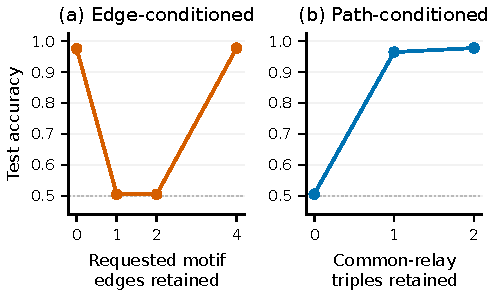
\includegraphics[width=\linewidth]{figures/edge_vs_path.pdf}
\caption{\textbf{Different structural doses can hide source-transport
differences.} (a) Requested retention of named motif edges on a real $k=4$
subgraph gives a nonmonotone response. (b) A path-conditioned edit gives a
graded response. Both zero-dose reconstructions have zero common-relay
triples, despite their different accuracies. The panels are separate
archived experiments; error bars are ten-block bootstrap 95\% intervals.}
\label{fig:edge-path}
\end{figure}

Path conditioning changes the intervention. The base graph has two
enumerated triples, one for each sink. The constrained zero-, one-, and
two-triple graphs achieve $0.5055$, $0.9641$, and $0.9772$
(Fig.~\ref{fig:edge-path}b). The full-minus-zero difference is
$0.4717$ with interval $[0.4603,0.4824]$ and corrected $q=0.0036$.
The recorded terminal-set and degree/module checks all pass. Here the
two-triple and full settings are the same retained set, so they represent
one dose, not an additional replication.

The designs also differ in deletion order and randomized partner choices.
Their task-information contrast can be inspected directly through $T$.

\subsection{Question 1: does structural matching preserve information?}
\label{sec:replay}

The decisive comparison concerns two zero-common-relay reconstructions
with the same degree and module constraints. Their certificates agree, but
their transfers do not: named-edge compensation retains both sources through
separate relays, while path conditioning loses source $b$ at the readout.
Proposition~1 assigns ideal solvability only to the first. This is consistent
with archived accuracies 0.9745 and 0.5055. The matrices are reconstructed
from public MaleCNS tables and
archived extraction/intervention code. The recovered weight table matches
the original release's recorded byte count and SHA-256. The narrow base
matches 768 nodes, 44,906 dense edges, 3,072 retained edges, the five selected
motif body IDs, and the two recorded base common-relay triples. These are
post-hoc reconstruction checks; original runtime graph arrays and their
instance hashes were not retained.

Table~\ref{tab:core} places the reconstructed transfers beside the
corresponding archived outcomes. Columns of $T$ are ordered $(a,b)$ and
rows $(s_1,s_2)$.

\begin{table}[t]
\centering
\caption{\textbf{Zero common-relay count, different source access.}
Both zero-dose reconstructions preserve the base degrees/module counts
and have $|\mathcal C|=0$. Transfers are post-hoc recipe reconstructions;
accuracy and seed-bootstrap 95\% intervals are archived fit outcomes.
Original dose-instance hashes are unavailable.}
\label{tab:core}
\small
\begin{tabular}{@{}lccc@{}}
\toprule
Condition & $16T$ & Visible & Archived accuracy \\
\midrule
Base & $\left(\begin{smallmatrix}2&1\\2&1\end{smallmatrix}\right)$ & $a,b$ &
\shortstack{0.9772\\{[0.9727, 0.9820]}} \\[6pt]
Edge-zero & $\left(\begin{smallmatrix}1&0\\1&1\end{smallmatrix}\right)$ & $a,b$ &
\shortstack{0.9745\\{[0.9669, 0.9812]}} \\[6pt]
Path-zero & $\left(\begin{smallmatrix}1&0\\1&0\end{smallmatrix}\right)$ & $a$ &
\shortstack{0.5055\\{[0.4969, 0.5150]}} \\
\bottomrule
\end{tabular}
\end{table}

Both zero-dose graphs have $\mathcal C=\varnothing$ and preserve the
base degrees and module counts. The named-edge reconstruction retains
$a$ through relay 18 to both sinks and $b$ through relay 57 to $s_2$,
using compact node indices. No relay receives both sources on these
readout routes. By contrast, the path-conditioned reconstruction retains
the $a$ routes but has a zero $b$ column. Equation~\eqref{eq:criterion} assigns chance-level population accuracy
to this path-zero reconstruction. Edge-zero exposes both sources through
an invertible mixture and preserves the ideal label information.

The reconstructed source-access difference in Figure~\ref{fig:overview}
is consistent with the archived high/chance outcomes. Because both
reconstructions have the same empty common-relay family, the comparison
cannot attribute the historical gap specifically to the no-new-triple
rejection rule or isolate it from the other editing choices.

\subsection{Question 2: does information preservation predict finite use?}
\label{sec:multi}

When both sources remain visible, preservation of ideal information need
not imply comparable trained performance. The $k=8$ study uses broad and
narrow annotation predicates and requires
at least three enumerated triples per selected source--sink configuration.
Both extractions have exactly three, giving four distinct dose levels.
Every reported dose is feasible, retains the requested terminal set, and
has zero recorded degree/module-count violations. The same ten-block task
protocol is used throughout.

\begin{figure*}[t]
\centering
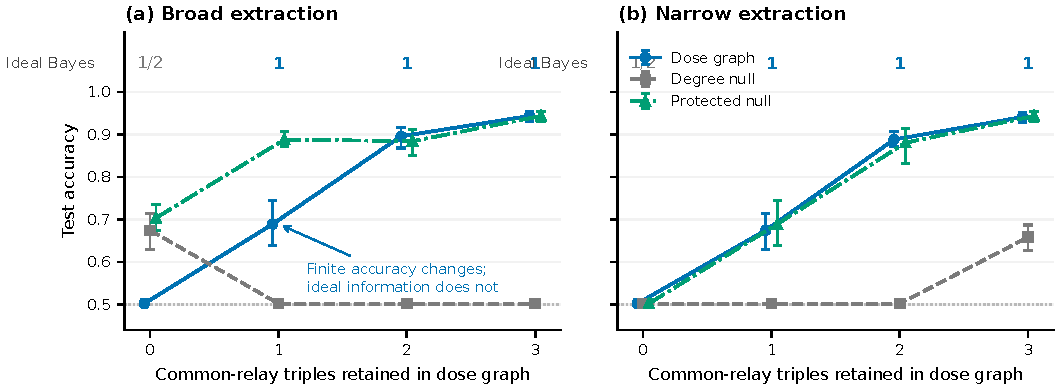
\includegraphics[width=0.86\textwidth]{figures/multigraph.pdf}
\caption{\textbf{Finite-readout accuracy varies among
information-preserving doses.} Blue, gray and green curves report archived dose, degree-null and
protected-null accuracies in both $k{=}8$ extractions. Error bars are
seed-block bootstrap 95\% intervals. Every nonzero dose retains both sources, so its ideal Bayes accuracy
is 1; only the zero dose is $1/2$. Null graphs are different counterfactuals
and are not assigned those ideal labels. All doses are from the same animal.}
\label{fig:multi}
\end{figure*}

The broad extraction's dose-graph accuracies are $0.5017$, $0.6889$,
$0.8955$, and $0.9432$ for zero through three triples
(Fig.~\ref{fig:multi}a). The narrow extraction gives $0.5017$,
$0.6742$, $0.8877$, and $0.9407$
(Fig.~\ref{fig:multi}b). Full-minus-zero gaps are $0.4415$
($[0.4265,0.4542]$, corrected $q=0.0025$) and $0.4390$
($[0.4249,0.4525]$, corrected $q=0.0036$), respectively.
Direct oracle readouts reach approximately $0.999$ and linear probes
remain near chance.

The intervention changes routes while holding degrees, module counts,
and the propagation/readout architecture fixed within each extraction.
It therefore holds more statistical quantities fixed than a density change.
The reconstructed $k=8$ operators also make the remaining distinction
explicit. Broad zero dose has $64T=\left(\begin{smallmatrix}0&0\\1&0\end{smallmatrix}\right)$,
while narrow zero dose has $T=0$; both lack one or both source classes.
Every nonzero dose exposes both sources, so Eq.~\eqref{eq:criterion}
assigns all of them Bayes accuracy one in the ideal task. Their mixture
geometry and coefficients vary (full matrices are in the supplement).
Thus the graded finite-readout accuracies vary within an
information-preserving regime, rather than quantifying successive losses
of population label information.

Agreement across the two extraction rules supports robustness to this
choice of visual-neuron predicate. Both use the same animal and task
family; their 195-neuron overlap is reported in Table~\ref{tab:graphs}.
The supplement retains all seed arrays and controls.

\subsection{Nulls answer different counterfactuals}
\label{sec:exceptions}

The protected null often retains task ability at the full dose: its broad
accuracy is $0.9432$, and its narrow accuracy is $0.9432$ compared with
the dose graph's $0.9407$. The latter paired graph-minus-null interval is
$[-0.0145,0.0087]$. This supports limited sensitivity to the remaining
wiring under those conditions. It does not establish equality of the
underlying functions.

More revealing are the conditions where protection is insufficient to
match behavior. In the broad zero-dose setting, the dose graph is at
$0.5017$, but the degree null reaches $0.6742$ and the protected null
$0.7032$. With no retained triples to protect, these are unrestricted
rewirings with different fixed graph-operation seeds. In the broad
one-triple setting, protection gives $0.8877$, well above the dose graph's
$0.6889$; the graph-minus-protected difference is $-0.1988$ with interval
$[-0.2483,-0.1413]$. The narrow full-dose degree null also retains
$0.6581$ accuracy.

The common-relay rejection rule
applies during dose construction, while subsequent null generation
protects a set of edges without restricting all new routes. The nulls'
task ability demonstrates that the two operations cannot be treated as
the same counterfactual. A protected null asks whether retaining those
edges allows the task after background rewiring; it does not certify
that only those edges explain the output. The two contrasts separate retaining selected routes from constraining
all surviving task information.

\subsection{Transfer geometry beyond two-source visibility}
\label{sec:images}

For the noiseless subspace XOR task, source visibility is sufficient for
ideal label solvability, even when the transfer columns are parallel. Visual
representations pose a different challenge: the relevant information must be
extracted from mixtures of image features. We therefore compare transfer rank
with finite-readout behavior under the same operator. We retrain the archived
readout architecture on the three reconstructed transfers, using the recorded
protocol: a $32\!\to\!64\!\to\!1$ ReLU MLP, Adam with learning rate
0.006, 120 epochs of 32 batches of 128, and the ten recorded seeds. With
features present only at $a$ and $b$, the sink input is exactly $TX_{ab}$.
The linear control uses the same budget with the hidden layer removed.

On the subspace XOR, this replay returns MLP accuracies 0.976, 0.979, and
0.504 for the base, named-edge, and path-zero graphs
(Table~\ref{tab:executed}). The archived fits were 0.9772, 0.9745, and
0.5055. Every linear readout stays near 0.505, including on the two graphs
where the MLP exceeds 0.97. The trained model follows source visibility. A linear readout of the transferred features remains near chance, even when ideal XOR solvability is preserved.

The visual task keeps that architecture and those seeds, and replaces the Gaussian
subspaces with handwritten digits~\cite{optdigits1998}. A fixed projection maps
each 32-pixel half to 16 dimensions. Source $a$ receives an upper half, source
$b$ a lower half drawn from an independent digit, and the label is the XOR of
the two digit parities. The MLP reaches 0.746 when the columns are independent,
0.663 when they are parallel, and 0.506 when the source-$b$ column is zero.
Linear readouts remain at chance on all three graphs. Retaining both
common relays therefore does not beat an invertible pair of separate routes.
The reverse-support CIFAR-10 subset remains a negative control
(gaps $-0.0044$ and $-0.0019$).

\begin{table}[t]
\centering
\caption{\textbf{Readout performance on reconstructed transfers.}
Means over ten seeds. The MLP is retrained from the archived architecture.
All three graphs share degree and module counts. Linear
accuracies are 0.506, 0.505, and 0.505 on the subspace task and 0.505,
0.502, and 0.506 on the visual task, in the same row order.}
\label{tab:executed}
\small
\setlength{\tabcolsep}{3pt}
\begin{tabular}{@{}lcccc@{}}
\toprule
Graph & $|\mathcal C|$ & rank & Subspace & Visual \\
\midrule
Base & 2 & 1 & 0.976 & 0.663 \\
Named-edge zero & 0 & 2 & 0.979 & 0.746 \\
Path zero & 0 & 1 & 0.504 & 0.506 \\
\bottomrule
\end{tabular}
\end{table}

\subsection{Multi-source geometry on visual codes}
\label{sec:population}

The two-source XOR task is a setting in which visibility alone determines
ideal label solvability. We now ask for the class of one designated image
in a mixture of four independently sampled visual representations
(Fig.~\ref{fig:geometry}). Source visibility and independent source recovery are distinct properties.
We characterize the latter through the private energy defined in
Eq.~\eqref{eq:private}.
A two-convolution network is trained on $30{,}000$ CIFAR-10 images and then
frozen. Its $16$-d embedding is linearly classified at $0.571$ on the official
$10{,}000$-image test set. Sources $\{109,107,152,6\}$ receive independent
images through the same operator and sinks. The label is the class at one
source, so chance is $0.1$. The readout is a $32\!\to\!64\!\to\!10$ MLP, plus
a linear control, for ten seeds. Each accuracy resamples $2{,}048$ test
images. On the named-edge graph, half the energy of source $109$ lies outside
the other three columns. The base column has twice that energy and no private
component. Path zero removes it. Source $107$ keeps a shared high-gain column
on every graph.

\begin{table}[t]
\centering
\caption{\textbf{CIFAR-10 identity from four simultaneous images.} Chance is
$0.1$. A linear probe of the isolated embedding scores $0.571$. Private energy
is the squared norm of the target column's orthogonal residual. The transfer
column of source $109$ vanishes under path conditioning.}
\label{tab:population}
\small
\setlength{\tabcolsep}{4pt}
\begin{tabular}{@{}llccc@{}}
\toprule
Label & Graph & $\rho_j$ & MLP & Linear \\
\midrule
109 & Base & 0 & 0.164 & 0.166 \\
109 & Named-edge zero & 0.00195 & 0.566 & 0.558 \\
109 & Path zero & 0 & 0.096 & 0.098 \\
107 & Base & 0 & 0.281 & 0.277 \\
107 & Named-edge zero & 0 & 0.441 & 0.434 \\
107 & Path zero & 0 & 0.440 & 0.434 \\
\bottomrule
\end{tabular}
\end{table}

Source $109$ gains a nonzero private component under named-edge compensation:
MLP accuracy is $0.566$, against $0.164$ on the base graph and $0.096$ when
its column vanishes. The linear control reaches $0.558$, beside the $0.571$
linear probe of the unmixed embedding. Source $107$ stays readable without a
private component, at $0.440$ on path zero, so class information can survive
when exact source recovery cannot. The UCI digit split is $0.852$, $0.099$,
and $0.698$ for the same three conditions.

\begin{figure}[t]
\centering
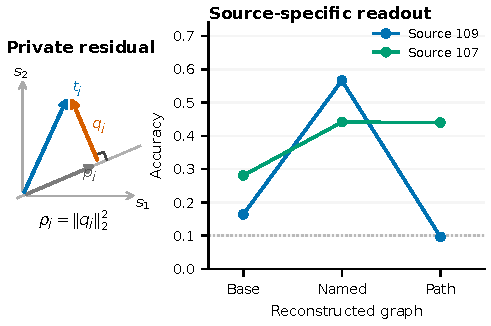
\includegraphics[width=0.92\linewidth]{figures/transfer_geometry.pdf}
\caption{\textbf{Independent source access and visual readout.}
Left: for a one-dimensional competing subspace, the target column $t_j$
splits into its projection $p_j$ and an orthogonal residual $q_j$. A nonzero
residual permits exact linear recovery of that source under noiseless mixing.
Right: ten-seed MLP accuracies for two CIFAR-10 sources. Source 109 gains a
private component under named-edge compensation; source 107 stays readable
through a shared mixture.}
\label{fig:geometry}
\end{figure}

\section{Discussion}
\label{sec:discussion}

\paragraph{What the audit adds.}
The counterexample separates a structural certificate from the computation
that replaces the removed structure. Separate routes expose both sources in
one reconstruction; the other loses a source at the readout. The transfer
makes this difference explicit and complements boundary-aware
controls~\cite{park2026}. Its contribution is the audit protocol and the
evidence that the two levels can disagree, rather than a new graph
architecture or a universal information law.

\paragraph{What the criterion guarantees.}
Proposition~1 is a population statement for one noiseless subspace task.
It says whether the XOR label is decodable from transferred source states;
it does not promise finite-MLP accuracy or biological generality.

\paragraph{Information is not utilization.}
All nonzero $k=8$ doses preserve ideal label information, while finite
accuracy varies substantially. Those curves describe how the recorded
procedure handles different input mixtures within an information-preserving
regime. Rank-one transfer can retain the label, so full source recovery is a
stronger requirement than this classification task needs.

\paragraph{Validity boundary.}
The evidence comes from one male connectome, two overlapping $k{=}8$
extractions, a fixed two-step linear operator and synthetic task labels.
The CIFAR-10 assay tests source-specific readouts on four mixed codes, not
recognition accuracy. The exact population criterion assumes noiseless
continuous features; nonlinear propagation requires an input-dependent
analysis. The two dense $k{=}8$ bases match frozen source hashes, but
historical dose-instance hashes and bit-identical initializations are
unavailable. Reconstructed matrices therefore give a consistency result,
and the historical gap cannot be assigned to one editing rule. A separate
reverse-support image control finds no connectome-specific benefit.

\section{Conclusion}
\label{sec:conclusion}

Graph interventions should report the information that survives at the
readout alongside the structure they preserve. The task-information audit
uses the executed operator to expose source access, transfer geometry and
their consequences for an ideal task, then keeps finite-model accuracy as a
separate measurement. On matched MaleCNS graphs, this protocol reveals
different information under the same structural certificate and shows that
information-preserving edits can still produce different learned behavior.
The result is a sharper standard for intervention studies: state the
operator, inspect the information reaching the readout, and report which
level of the analysis supports each conclusion.

\clearpage
\section*{LLM Usage Statement}
AI tools assisted with evidence synthesis, scientific framing, code inspection,
reference verification, reanalysis of recorded results, figure preparation,
and drafting and editing the manuscript. New readout comparisons trained the
archived MLP architecture and linear controls on reconstructed transfers,
including the CIFAR-10 identity assay and digit-identity comparison.
Original archived weights were not reloaded. The authors take responsibility
for the content, including the interpretation of archived experiments and
the accuracy of the references.
{\small\bibliographystyle{ieeenat_fullname}\bibliography{references}}
\end{document}
